\documentclass[12pt]{article}

\pagestyle{empty}
\setcounter{secnumdepth}{4}
\setcounter{tocdepth}{4}

\topmargin=0cm
\oddsidemargin=0cm
\textheight=22.0cm
\textwidth=16cm
\parindent=0cm
\parskip=0.15cm
\topskip=0truecm
\raggedbottom
\abovedisplayskip=3mm
\belowdisplayskip=3mm
\abovedisplayshortskip=0mm
\belowdisplayshortskip=2mm
\normalbaselineskip=12pt
\normalbaselines
\usepackage[table]{xcolor}
\usepackage{caption}
\usepackage{graphicx}
\usepackage{enumitem}
\usepackage{etoc}
\usepackage{blindtext}

\begin{document}

\graphicspath{{C:/Users/Marc/Desktop/ReqDocFolder/}}

\vspace*{0.5in}
\centerline{\bf\Large Requirements Document}

\vspace*{0.5in}
\centerline{\bf\Large Team PI-B}

\vspace*{0.5in}
\centerline{\bf\Large 9 February 2020}

\vspace*{1.0in}
\centerline{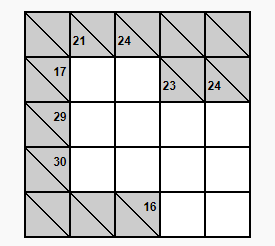
\includegraphics[scale=.75]{KakuroTemp.png}}
\centerline{\bf\Large Kakuro}

\vspace*{0.5in}
\begin{table}[htbp]
\begin{center}
\caption*{Team members}
\begin{tabular}{|c | c|}
\hline
\cellcolor{gray}Name & \cellcolor{gray}ID Number \\
\hline
Sajib Ahmed & 40044867 \\
\hline
Yaroslav Bilodid & 40068605 \\
\hline
Jesse Desmarais & 40035761 \\
\hline
Antoine Farley & 40100554 \\
\hline
Marc Hegedus & 26242219 \\
\hline
Katerina Tambakis & 27010486 \\
\hline
Yingjie Zhou & 26433820 \\
\hline
\end{tabular}
\end{center}
\end{table}

\newpage
\pagestyle{plain}
\tableofcontents

\newpage
\pagestyle{plain}
\section{System}
\subsection{Introduction}

\hspace{\parindent} The purpose of this document is to demonstrate the requirements needed to build the computer puzzle game Kakuro. Kakuro, typically a single player game, is a kind of logic puzzle that is often referred to as a mathematical transformation of the crossword puzzle. Kakuro is typically played on a 10x10 grid filled with black and white cells. The black cells contain a diagonal slash from upper-left to lower-right and a number in one or both halves, such that each horizontal entry has a number in the black half-cell to its immediate left and each vertical entry has a number in the black half-cell immediately above it. These numbers are commonly called clues. The objective of the puzzle is to insert a digit from 1 to 9 inclusive into each white cell such that the sum of the numbers in each entry matches the clue associated with it and that no digit is duplicated in any entry. 

\subsection{Purpose}

\hspace{\parindent} The purpose of the Software Requirements Document describes the specification of the Kakuro puzzle game, which is in partial fulfillment of the requirements of COMP 354. This document will define the requirements of the user interface, the product functions, actors, non-functional constraints, data definition, and model for this application. The model will include use case diagrams and domain model UML diagrams. Furthermore, a detailed project plan will be provided, including the schedule of the upcoming phases. This document will serve as a basis for the upcoming phases for this project. 

\subsection{Context}

\hspace{\parindent} This document addresses the requirements that will be used as a basis for the design phase. A number of figures will be provided to demonstrate how the game will appear at completion along with its special features such a difficulty level. The actors will include the target audience and environment required for this game. The model will demonstrate the use cases and its domain model UML diagram explaining the relationship of the actors with one another. Finally, a chart will include the breakdown of the amount of time logged into developing the project from all different tasks. 

\subsection{Business Goals}

\hspace{\parindent} Our objective of developing kakuro is in relation to the growth of PI-B. We are thriving to fulfill the customer’s needs so that we can expand our business portfolio in order to reach other customers’ business. Moreover, we hope to achieve a high number of downloads in order to catch the eye of advertisers that wish to participate in future projects that will be given to us.


\pagestyle{plain} 
\section{Domain Concepts}
\subsection{Objectives}

The project to be completed in COMP 354 of Winter 2020 is to create a functional replica of the puzzle game Kakuro. Team PIB's version in iteration one will consist of a singular solvable puzzle. Functionality will be limited to input from the client and feedback for the verification of a correct solution. The main objective is to apply software engineering techniques for the development process to be test-driven, agile, and object-oriented. There will be three iterations, each having their own deadlines. Efficient management and communication amongst our group is understood to be central in accomplishing the required tasks. The client wants the following as deliverables for the first iteration: a basic graphical user interface, a model-view-controller architecture coded in Java, and a categorized set of use cases.\\  
The three iterations will each have a document to be handed in to the client. The information regarding their naming, deliverables, and dates are tabulated below:\\

\begin{table}[htbp]
\begin{center}
\begin{tabular}{| c | c | c |}
\hline
\cellcolor{gray}Iteration & \cellcolor{gray}Deliverable & \cellcolor{gray} Date \\
\hline
Requirement & Requirements Document & 2020/02/09 \\
\hline
Design & Design Document & 2020/03/15 \\
\hline
Implementation & Final Document & 2020/04/5 \\
\hline
\end{tabular}
\caption*{\textit {Project Timeline}}
\end{center}
\end{table}


\subsubsection{Kakuro Puzzle Game Specifications}

Kakuro is a japanese mathematical logic puzzle with rules similar to the crossword and sudoku. To develop a successful graphical user interface, the game's rules and characteristics are to be clearly detailed. This will allow clients and various actors to recognize the product for an intuitive feel. Due to the simplistic nature of the game, development will be focused on limiting user interaction and increasing response. This will be realized in the form of input validation. Users will interact with a single interface where numerals from one to nine are to be entered. If incorrect, a red translucent overlay will be superimposed upon the respective tile. A thorough description of Kakuro's mechanics is provided below. \\

\newpage
\pagestyle{plain}
\paragraph{Gameboard}\hfill\\ 
\hfill\\
Kakuro's classic form is composed of a monochromatic square matrix where three different tiles are displayed. They are the following: blank, input, and clue. Blank tiles are black and cannot contain any value. Clients are to interact only with the input tile. Numerical values will be inserted to complete the sums found within the clue tiles. Clue tiles are bisected diagonally where the lower and higher sums must correspond to the addition of all the vertically and horizontally aligned numerals in the input tiles, respectively. Input tiles along a specified direction can only have unique values from 1 to 9. Their intersections must then contain the same numeral. As such, a solution is obtained when every sum has been rightfully achieved throughout the gameboard matrix. The figure below shows a Kakuro puzzle at the easy difficulty.\\

\begin{figure}[htbp]
\centerline{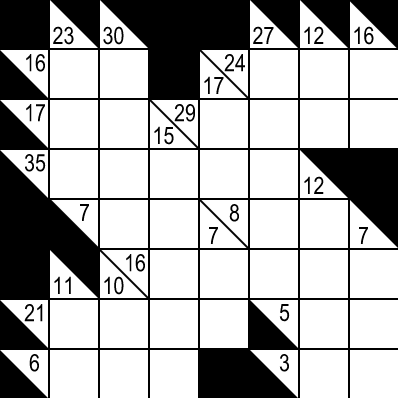
\includegraphics[scale=.6]{gameboard.png}}
\centerline{\textit {Easy Kakuro gameboard}}
\end{figure}

\paragraph{Tiles}\hfill\\ 
\hfill\\ 
The three distinct types of tiles are shown in the figure below in the given order: blank, input, and clue. Blank tiles are always filled with black and no numeral is ever shown within its confines. Input tiles are white and users are to fill them with a number from one to nine. Clue tiles are bisected from the top left to the bottom right and come in three separate formats. If a corner is white a sum will shown, whereas if it's black none will appear. As such, both corners may be hold a sum, or only one of the two might. \\ 

\begin{figure}[htbp]
\centerline{
\includegraphics[scale=.75]{tilevariation.png}}
\centerline{\textit {Tile variation as seen in Kakuro}}
\end{figure}

\newpage
\pagestyle{plain} 
\paragraph{Sum and intersections}\hfill\\ 
\hfill\\
A vertical and horizontal column has been filled out with a possible solution to the gameboard shown in section 2.1.1.1. The top of the vertical column suggests a sum of 30 is needed from the input tiles vertically below. A combination of 9-8-7-6 must be placed within the four allotted slots. This vertical column had two clues where the second formed a break. Clue tiles that appear sequentially along a particular column represent a new sum to acquire from the input tiles. The second reads a sum of 10. A combination of 9-1, 8-2, 7-3, or 6-4 is allowed to be placed. The horizontal that has been filled shares a tile with the vertical column. This is called an intersection. The number in that input tile must be correct for both columns. The horizontal's first number is 7. Since a there lies a 6, only a 1 can be placed within the adjacent tile. The flow of the game concerns itself by correctly forming the proper sums and accommodating the many intersections between columns.\\

\begin{figure}[htbp]
\centerline{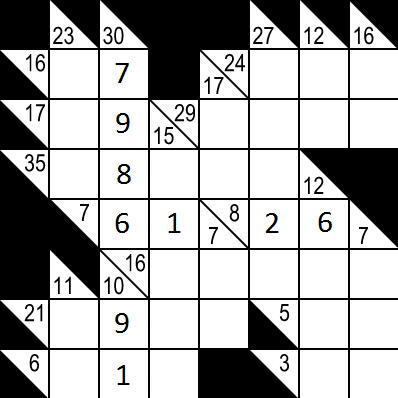
\includegraphics[scale=.6]{gameboardpartial.png}}
\centerline{\textit {Partially completed Kakuro gameboard}}
\end{figure}

\newpage
\pagestyle{plain}
\paragraph{Solution}\hfill\\ 
\hfill\\
The final solution to the gameboard shown in section 2.1.1.1 is given below. Each of the following requirements has been met:

\begin{description}[font=$\bullet$~\normalfont\scshape\color{red!50!black}]
\item [Numerals] Numbers used within the input tiles are limited from 1 to 9.
\item [Sum] Every input tile along a column corresponds to its vertical and/or horizontal clue tile. 
\item [Intersection] Every intersection between vertical and horizontal columns had a common numeral that worked towards the respective sum.
\item [Completion] Every input tile has been correctly filled out in the gameboard matrix.
\end{description}

The difficulty is set to easy due to the clues being too telling of the numbers needing to be entered. Taking a look at the top left, there's only one variation of numbers which can be inserted. This forms a good base to complete the rest of the puzzle.\\


\begin{figure}[htbp]
\centerline{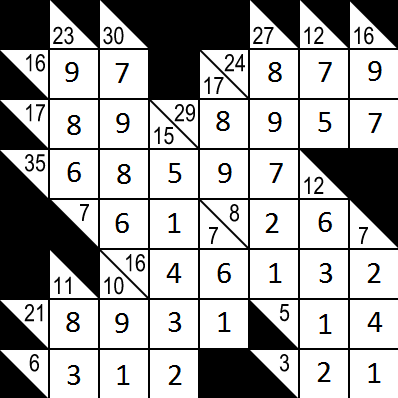
\includegraphics[scale=.6]{gameboardsol.png}}
\centerline{\textit {Kakuro gameboard solution}}
\end{figure}


\newpage
\pagestyle{plain} 
\subsection{Domain Model UML}
In test driven development progression is measured through the completion of use cases. The methodology is also aimed to be agile, favouring short cycles or iterations. For the first iteration base functionality is to be implemented. The following UML depicts several use cases that are currently part of the problem domain:\\

\begin{figure}[htbp]
\centerline{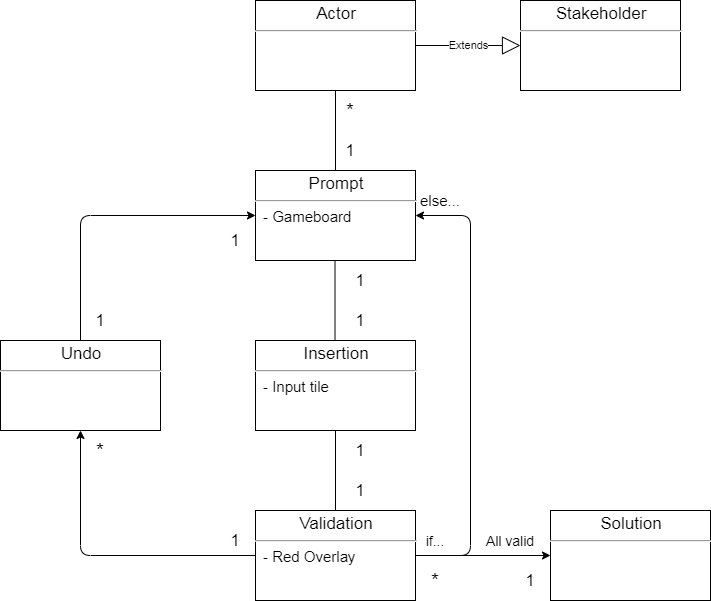
\includegraphics[scale=.6]{TempUML.png}}
\centerline{\textit {Problem Domain UML}}
\end{figure}

\newpage
\pagestyle{plain} 
\section{Actors}

Stakeholders are those who would show interest in a product, for example, through marketing. Actors form a subset from those that directly interact with the product. In the first iteration of the Kakuro puzzle, actors come in the given forms:

\begin{description}[font=$\bullet$~\normalfont\scshape\color{red!50!black}] 
\item [Coders] In a test driven design, code is tested in segments to implement functionality.
\item [Documenters] Through communication and verification, a requirements document can be written as a deliverable to the client.
\item [Organizers] To keep a steady purposeful work flow, one must keep track and organize the trajectory of the project by interacting with the coder's work.    
\item [Quality Assurance] The improvement of the code's structure and design is validated by an interaction.
\item [Players] Once base functionality is attained, users may willing play through a puzzle. 
\end{description}

\newpage
\pagestyle{plain} 
\section{Use Cases}

In the first iteration, the user and system need only interact to the point where base functionality is achieved. The use case diagram below depicts the requirements and scope of the system.

Use cases 1 and 2 are system functions relayed to the player and should not need validation to operate. Whereas with use cases 3 and 4, information from the player is relayed to the system. For example, the former sends feedback to the player if the value entered is incorrect.


\subsection{Overview}

\begin{figure}[htbp]
\centerline{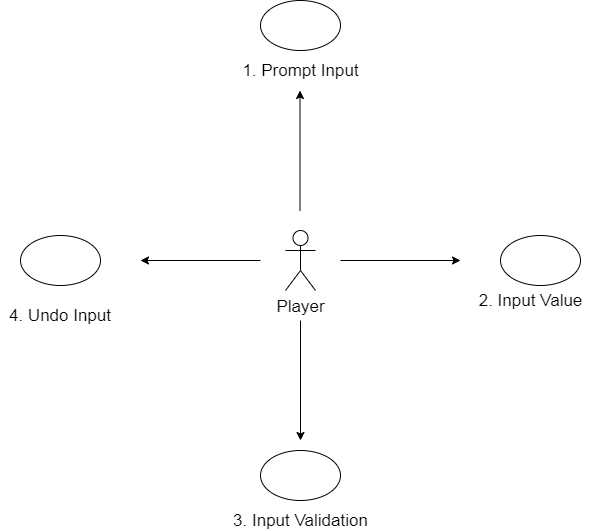
\includegraphics[scale=.6]{Usecase Diagram.png}}
\centerline{\textit {Use Case Diagram}}
\end{figure}

\newpage
\pagestyle{plain} 
\subsubsection{Use Case 1: Prompt Input} \label{uc:1}

\begin{table}[htbp]
\begin{center}
\begin{tabular}{| c | m{10cm} |}
\hline
\cellcolor{lightgray}Description & Signals user to enter values. \\
\hline
\cellcolor{lightgray}Summary & A Kakuro puzzle is displayed. \\
\hline
\cellcolor{lightgray}Actors & Player \\
\hline
\cellcolor{lightgray}Pre-conditions &
\begin{description}[font=$\bullet$~\normalfont\scshape]
\item Player starts a game.
\end{description}\\
\hline
\cellcolor{lightgray}Main Scenario & 
\begin{description}
\item [1.]Player starts a game.
\item [2.]A Kakuro puzzle is displayed. 
\item [3.]Input tiles represent a location where numerals may be accepted.
\end{description}\\
\hline
\cellcolor{lightgray}Exceptions & None \\
\hline
\cellcolor{lightgray}Post-Conditions & 
\begin{description}[font=$\bullet$~\normalfont\scshape]
\item The Kakuro puzzle prompts input until a solution is found.
\end{description}\\
\hline
\cellcolor{lightgray}Priority & Must have \\
\hline
\cellcolor{lightgray}Traces to Test Cases & None \\
\hline
\end{tabular}
\end{center}
\end{table}

\newpage
\pagestyle{plain} 
\subsubsection{Use Case 2: Input Value} \label{uc:1}

\begin{table}[htbp]
\begin{center}
\begin{tabular}{| c | m{10cm} |}
\hline
\cellcolor{lightgray}Description & Allows user to enter a numeral.\\
\hline
\cellcolor{lightgray}Summary & User may input numerals in input tiles to form a solution. \\
\hline
\cellcolor{lightgray}Actors & Player \\
\hline
\cellcolor{lightgray}Pre-conditions &
\begin{description}[font=$\bullet$~\normalfont\scshape]
\item Player's turn to act.
\item Tile selected is an input tile. 
\end{description}\\
\hline
\cellcolor{lightgray}Main Scenario & 
\begin{description}
\item [1.]Player starts a game.
\item [2.]Player selects an input tile. 
\item [3.]Player enters a value.
\end{description}\\
\hline
\cellcolor{lightgray}Exceptions & None \\
\hline
\cellcolor{lightgray}Post-Conditions & 
\begin{description}[font=$\bullet$~\normalfont\scshape]
\item A value now shows within a played input tile.
\end{description}\\
\hline
\cellcolor{lightgray}Priority & Must have \\
\hline
\cellcolor{lightgray}Traces to Test Cases & None \\
\hline
\end{tabular}
\end{center}
\end{table}

\newpage
\pagestyle{plain} 
\subsubsection{Use Case 3: Input Validation} \label{uc:1}

\begin{table}[htbp]
\begin{center}
\begin{tabular}{| c | m{10cm} |}
\hline
\cellcolor{lightgray}Description & Allows user to receive feedback on a number entered in an input tile. \\
\hline
\cellcolor{lightgray}Summary & A number is entered from 1 to 9 in an input tile and a red overlay is presented if incorrect. \\
\hline
\cellcolor{lightgray}Actors & Player \\
\hline
\cellcolor{lightgray}Pre-conditions &
\begin{description}[font=$\bullet$~\normalfont\scshape]
\item Player's turn to act.
\item Input tile is playable. 
\item The gameboard has not been solved.
\end{description}\\
\hline
\cellcolor{lightgray}Main Scenario & 
\begin{description}
\item [1.]Player selects an input tile.
\item [2.]The player enters an incorrect number. 
\item [3.]A red overlay on the input tile is displayed.
\end{description}\\
\hline
\cellcolor{lightgray}Exceptions & None \\
\hline
\cellcolor{lightgray}Post-Conditions & 
\begin{description}[font=$\bullet$~\normalfont\scshape]
\item A red overlay is now showing.
\item Player has feedback that the number is incorrect.
\end{description}\\
\hline
\cellcolor{lightgray}Priority & Must have \\
\hline
\cellcolor{lightgray}Traces to Test Cases & None \\
\hline
\end{tabular}
\end{center}
\end{table}

\newpage
\pagestyle{plain} 
\subsubsection{Use Case 4: Undo Input} \label{uc:2}

\begin{table}[htbp]
\begin{center}
\begin{tabular}{| c | m{10cm} |}
\hline
\cellcolor{lightgray}Description & Allows user to undo a numeral entered in an input tile. \\
\hline
\cellcolor{lightgray}Summary & User enters a numeral in an input tile. Undo removes the entered numeral from the gameboard matrix. \\
\hline
\cellcolor{lightgray}Actors & Player \\
\hline
\cellcolor{lightgray}Pre-conditions &
\begin{description}[font=$\bullet$~\normalfont\scshape]
\item Player's turn to act.
\item A numeral has been entered on the gameboard matrix 
\item The gameboard has not been solved.
\end{description}\\
\hline
\cellcolor{lightgray}Main Scenario & 
\begin{description}
\item [1.]User has entered a numeral within an input tile.
\item [2.]The numeral has the option to be undone.
\item [3.]The numeral is removed from the current input tile.
\end{description}\\
\hline
\cellcolor{lightgray}Exceptions & None \\
\hline
\cellcolor{lightgray}Post-Conditions & 
\begin{description}[font=$\bullet$~\normalfont\scshape]
\item Last played numeral is no longer on the gameboard matrix.
\item A previously entered numeral is present on the gameboard matrix.
\item Numerals may be removed until all input tiles are cleared.
\end{description}\\
\hline
\cellcolor{lightgray}Priority & Good to have \\
\hline
\cellcolor{lightgray}Traces to Test Cases & None \\
\hline
\end{tabular}
\end{center}
\end{table}

\newpage
\pagestyle{plain} 
\section{Non-Functional Constraints}
There are a couple of non-functional constraints that comes along with this project. Considering that the majority of PC’s of the players run either on Windows or Mac OS, one constraint is that the application Kakuro must be built in a language that is supported by these operating systems. The programming language chosen to create this game is Java. Another constraint is that the game will only be functional on desktops and laptops as it has not been adjusted to function on mobile devices. Lastly, the application must be updated time to time if there are updates to the operating systems to make sure the game is still compatible.\\

\newpage
\pagestyle{plain} 
\section{Data Dictionary}

\begin{table}[htbp]
\begin{tabular}{|c | m{10cm}|}
\hline
\cellcolor{gray}Name & \cellcolor{gray}Definition \\
\hline
Domain Model & Package that contains class and activity diagrams  \\
\hline
UML Diagram & Unified modeling language diagram that visually represents a system along with its main actors and actions \\
\hline
Use Cases & A description on how a person will proceed to complete an action \\
\hline
Actor & People who directly interact with the product \\
\hline
Stakeholder & People who show interest in the product\\
\hline
Non Functional Constraint & Attribute that a product contains that prevents it from functioning\\
\hline

\end{tabular}
\end{table}

\newpage
\pagestyle{plain}
\section{References (APA)}

Kakuro. (2019, December 18). Retrieved from https://en.wikipedia.org/wiki/Kakuro
\newpage
\pagestyle{plain} 
\appendix

\section{Description of File Format: Tasks}

Not Applicable.

\section{Description of File Format: Persons}

Not Applicable.

\end{document}
